\chapter*{Metodologia}

\section*{Função do Receptor}
\subsection*{Dados Geofísicos}

No âmbito do projeto SUBSAL, realizado conjuntamente entre o Observatório Nacional e a Petrobras,  instalou-se 24 estações sismográficas temporárias banda larga (STS2 ou Reftek RT151-120s). A faixa de frequência registrada varia de 50 Hz até 100 segundos.  As estações foram dispostas geometricamente em trẽs perfis em relação à costa, dois perpendiculares à costa, perfil 1 a oeste e perfil 2 a leste, e um paralelo, perfil 3, como observado na Figura \ref{figura1}. O perfil 1 estende-se da estação STA01, localizada próximo à costa, até a STA09. O perfil 2 vai da estação STA10, ao norte, até a STA16, próximo à costa. O perfil 3 é da estação STA17, oeste, até a STA24, leste. A distância entre as estações é aproximativamente de 20 km. As coordenadas das estações são dadas na Tabela \ref{tabela1}. 

\begin{figure}[!ht]
\centering
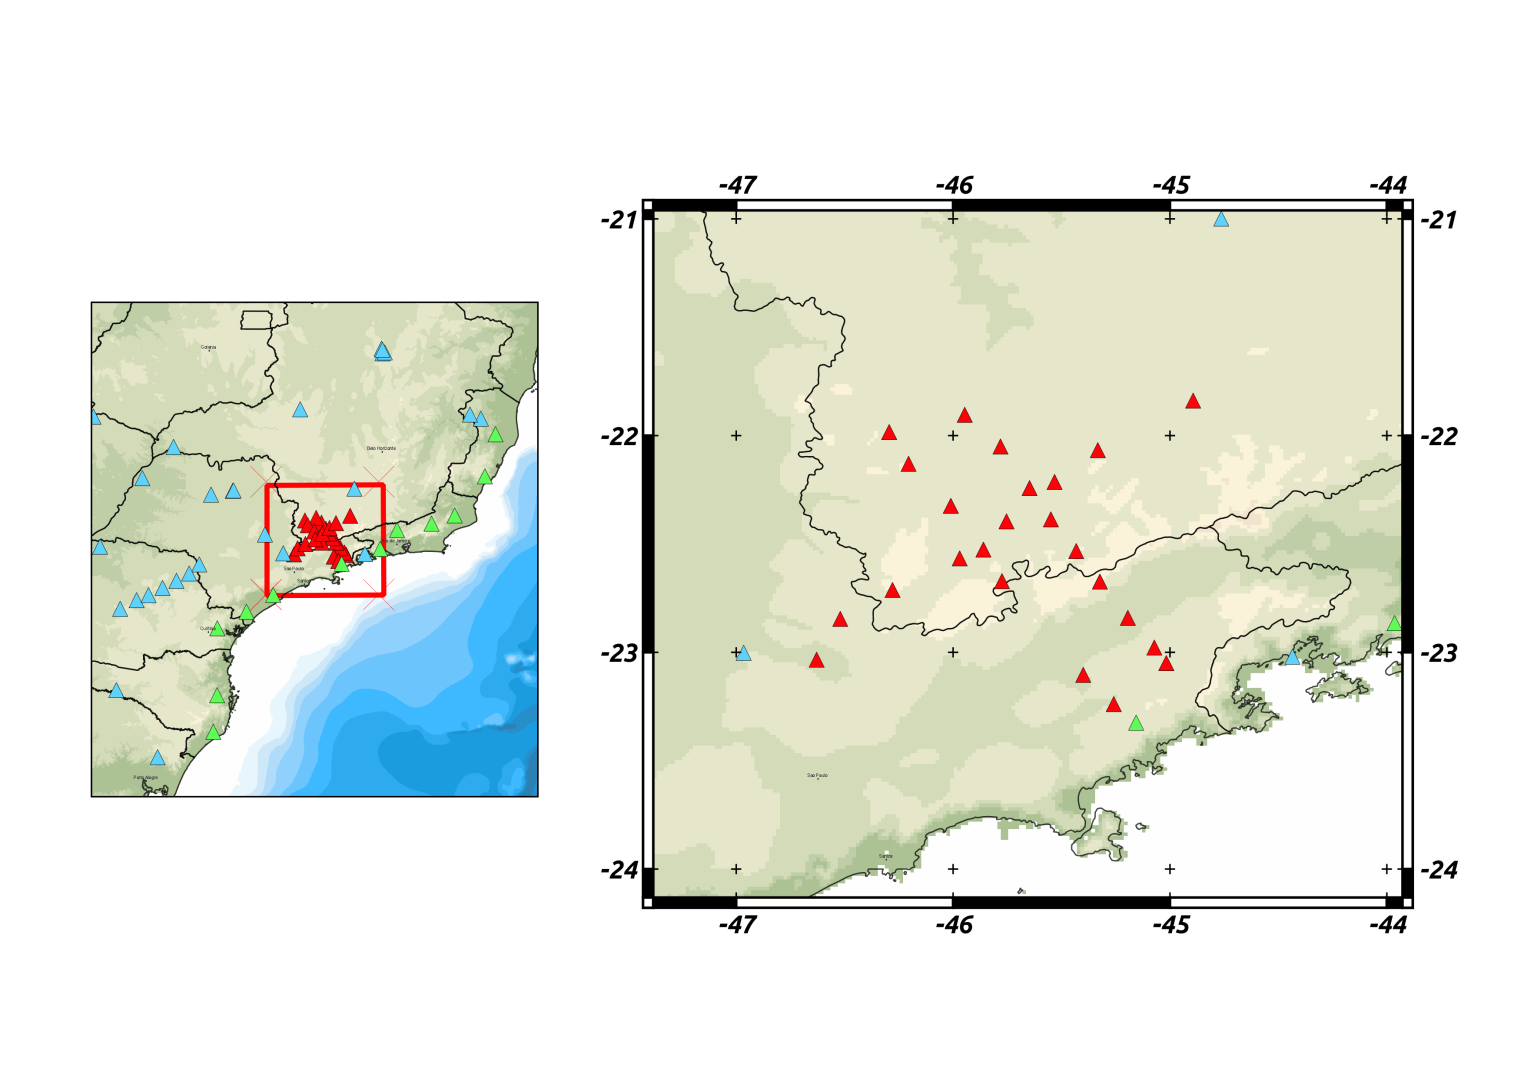
\includegraphics[scale=1]{mapa_das_estacoes_simosgraficas_instaladas.png}
\caption{Mapa das estações sismográficas instaladas (triângulos vermelhos). Os outros triângulos são estações da Rede Sismográfica Brasileira.}
\label{figura1}
\end{figure}

O período de operação das estações foi distinto para os perfis. Os dois perfis perpendiculares à costa foram instalados no meio do ano de 2012 e o perfil paralelo no final de 2012. As estações ficaram em fucionamento até o final do ano de 2013 registrando o movimento do terreno de maneira contínua. O produto do deslocamento das partículas é registrado pelo sismógrafo, através de sensores verticais e horizontais, em três componentes. Esse registro das componentes é chamado de sismograma. 

\begin{center}
\begin{table}[!ht]
\caption{Tabela com as coordenadas(Lat Long) e altitude (m) das Estações.}
\begin{center}
\begin{tabular}{| c | c | c | c |}
\toprule
{\large \textbf{Nome}} &	{\large \textbf{Latitude}} & {\large \textbf{Longitude}} & {\large \textbf{Elevação(m)}}\\
\bottomrule
STA01 & -23.049408 & -45.016808 & 950\\
STA02 & -22.977707 & -45.072017 & 886\\
STA03 & -22.840839 & -45.194141 & 576\\
STA04 & -22.673525 & -45.323162 & 902\\
STA05 & -22.5325 & -45.432383 & 1100\\
STA06 & -22.386261 & -45.549086 & 931\\
STA07 & -22.241667 & -45.647361 & 988\\
STA08 & -22.050056 & -45.781374 & 884\\
STA09 & -21.903929 & -45.946331 & 1045\\
STA10 & -21.98335 & -46.29471 & 1135\\
STA11 & -22.12999 & -46.20536 & 1455\\
STA12 & -22.32379 & -46.01047 & 890\\
STA13 & -22.52571 & -45.86029 & 918\\
STA14 & -22.67147 & -45.77467 & 974\\
STA15 & -23.10378 & -45.39983 & 895\\
STA16 & -23.2387 & -45.25919 & 906\\
STA17 & -23.0337 & -46.62914 & 776\\
STA18 & -22.84539 & -46.52033 & 957\\
STA19 & -22.71192 & -46.27943 & 1413\\
STA20 & -22.56621 & -45.96951 & 908\\
STA21 & -22.39548 & -45.75364 & 957\\
STA22 & -22.21361 & -45.53215 & 1052\\
STA23 & -22.06692 & -45.33267 & 993\\
STA24 & -21.83834 & -44.89324 & 995\\
\hline
\end{tabular}
\label{tabela1}
\end{center}
\end{table}
\end{center}

\begin{figure}[!ht]
\centering
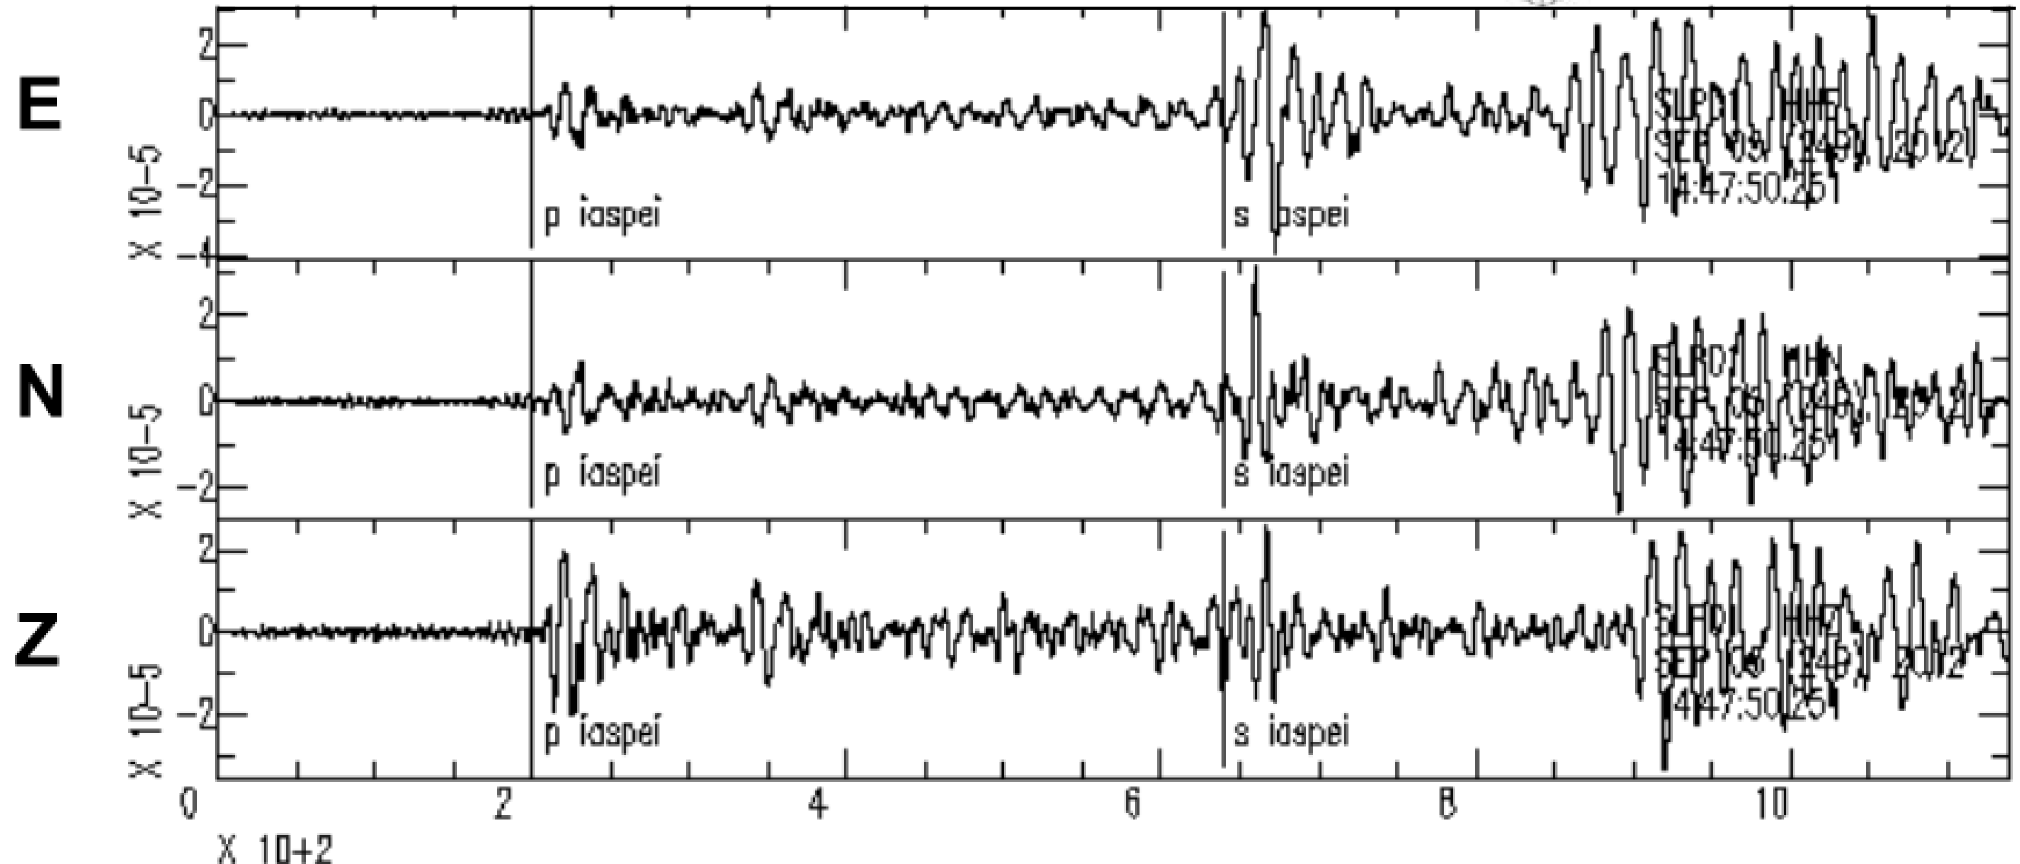
\includegraphics[scale=0.6]{sismograma.png}
\caption{Mapa das estações sismográficas instaladas (triângulos vermelhos). Os outros triângulos são estações da Rede Sismográfica Brasileira.}
\label{figura2}
\end{figure}

\subsection*{Fundamentos Teóricos}

A primeira análise feita é do nível de ruído nas estações usando o software PQLX. O cálculo do nível de ruído é baseado no trabalho de McNamara and Buland (2004). Os dados são cortados em intervalos de uma hora com 50% de superposição. Cada intervalo de uma hora está separado em 13 intervalos com 75% de superposição para calcular a “Power Spectral Density”. As médias obtidas para cada um dos 13 intervalos são usadas para estimar a “Probability Density Functions”, que são estimadas pelo cálculo das médias pelo número total de intervalos em hora. 

Esse método difere dos métodos utilizados normalmente porque não é necessário visu-
alizar todos os dados para remover o ruído existente, como sismos de calibração, ruídos
culturais, problemas instrumentais e falta de dados. Porque esse tipo de ruído terá uma
probabilidade muito baixa, segundo McNamara and Buland (2004).
Para calcular a espessura crustal na região utilizou-se o método da Função do Receptor
que foi desenvolvido por Langston (1977). Tal método faz uso do sinal de tele-sismos,
geradores de ondas planas de incidência quase-vertical embaixo de uma dada estação. A
onda P chega na discontinuidade de Moho e se decompõe em uma onda P transmitida e
uma onda S convertida. A diferença do tempo de chegada das duas ondas, onda S tem
velocidade inferior a onda P, e de outras reflexões permite inferir a profundidade de Moho,
como observado na Figura 1.2.
Sismos próximos, com distância menor que 20 graus da estação estudada, geram ondas
com incidência oblíqua e esse tipo de dado deve ser utilizado com um cuidado. Em sismos
com distâncias maiores que 95 graus as ondas P não chegam na estação devido a inversão
de velocidade no limite manto-núcleo, diminuição da velocidade da onda P entre o manto
e o núcleo, e não é observada a onda P direta.
No ínicio desse trabalho somente os dados de eventos incluídos no catálogo do IRIS
(Incorporated Research Institutions for Seismology) com magnitude maior que 5,5 entre
maio de 2011 e maio de 2012 foram disponibilizados. Mas agora utiliza-se dados coletados
do segundo semestre de 2013. A Figura 1.3 mostra eventos registrados na estação STA08.
A maior parte dos sismos registrados nas estações são eventos da cordilheira dos Andes
ou da América Central.

O processamento dos dados inclui a remoção da média e da tendência, e aplicou-se um filtro “High-pass” com freqüência de corte de 0.1 Hz para eventos com distância entre
20 e 95 graus e de 2 Hz para eventos próximos. Os dados originais com amostragens a
cada 0,01 segundos (100 Hz) são interpolados para gerar dados com amostragens cada
0,025 segundas (40 Hz), porque a informação de alta freqüência não é relevante nesse tipo
de análise.Os dados foram examinados visualmente para identificar e salvar o tempo de
chegada da onda P direta. Então as componente horizontais são rotadas para obter as
componentes “radial” e “transversal”.
As Funções do Receptor são calculadas com uma deconvolução no dominio do tempo

da componente radial pela componente vertical. Isso elimina partes similares dos sinais, a
fonte e a propagação da fonte até Moho, então a Função Receptor é sensível na delimitação
da estruturação superficial da crosta embaixo da estação. O programa SAC (Seismic
Analysis Code) foi usado para fazer o processamento e o cálculo das Funções Receptores. A
Figura 1.4 apresenta um exemplo da marcação da chegada da onda P direta, a componente
vertical e radial e a Função do Receptor registradas na estação STA08 em um dado evento.

Um método robusto de análise das Funções do Receptor é o método de Zhu and
Kanamori (2000). Usando as velocidades medianas na crosta, as diferenças de tempo
entre a P direta e a P convertida em S podem ser calculadas, bem como os tempos das
múltiplas.

Usando uma dada velocidade v p , os tempos de chegada podem ser calculados usando
a profundidade de Moho (H), a razão v p /v s e o parâmetro do raio, este é dependente
da localização do evento e da profundidade. Ao invés de tentar ajustar toda a função, o
método faz uma pesquisa, grid search, da espessura crustal e da razão v p /v s para calcular o
tempo de chegada teórico das ondas P convertidas em S e das múltiplas para cada registro.
A melhor combinação da espessura crustal e da razão v p /v s é aquela que maximiza o valor
das amplitudes reais das funções receptor.

Para obter uma imagem das discontinuidades, como por exemplo Moho, as Funções do
Receptor empilhadas são mapeadas em relação a posição da estação no perfil. Os dados
são separados em 4 grupos, segundo o azimute entre o sismo e a estação. A maioria do
eventos ocorrem na região noroeste e sudoeste, nota-se a escassez de eventos na região do
Oceano Atlântico. O objetivo dessa separação é avaliar se existem variações laterais de
estrutura.




\section*{Dispersão de Ondas de Superfície}
\subsection*{Dados Geofísicos}
\subsection*{Fundamentos Teóricos}